% $Id: template.tex 11 2007-04-03 22:25:53Z jpeltier $

\documentclass{vgtc}                          % final (conference style)
% \documentclass[review]{vgtc}                 % review
%\documentclass[widereview]{vgtc}             % wide-spaced review
%\documentclass[preprint]{vgtc}               % preprint
%\documentclass[electronic]{vgtc}             % electronic version

%% Uncomment one of the lines above depending on where your paper is
%% in the conference process. ``review'' and ``widereview'' are for review
%% submission, ``preprint'' is for pre-publication, and the final version
%% doesn't use a specific qualifier. Further, ``electronic'' includes
%% hyperreferences for more convenient online viewing.

%% Please use one of the ``review'' options in combination with the
%% assigned online id (see below) ONLY if your paper uses a double blind
%% review process. Some conferences, like IEEE Vis and InfoVis, have NOT
%% in the past.

%% Figures should be in CMYK or Grey scale format, otherwise, colour 
%% shifting may occur during the printing process.

%% These few lines make a distinction between latex and pdflatex calls and they
%% bring in essential packages for graphics and font handling.
%% Note that due to the \DeclareGraphicsExtensions{} call it is no longer necessary
%% to provide the the path and extension of a graphics file:
%% \includegraphics{diamondrule} is completely sufficient.
%%
\ifpdf%                                % if we use pdflatex
  \pdfoutput=1\relax                   % create PDFs from pdfLaTeX
  \pdfcompresslevel=9                  % PDF Compression
  \pdfoptionpdfminorversion=7          % create PDF 1.7
  \ExecuteOptions{pdftex}
  \usepackage{graphicx} % allow us to embed graphics files
  \usepackage{color}
  \DeclareGraphicsExtensions{.pdf,.png,.jpg,.jpeg} % for pdflatex we expect .pdf, .png, or .jpg files
\else%                                 % else we use pure latex
  \ExecuteOptions{dvips}
  \usepackage{graphicx}                % allow us to embed graphics files
  \DeclareGraphicsExtensions{.eps}     % for pure latex we expect eps files
\fi%

%% it is recomended to use ``\autoref{sec:bla}'' instead of ``Fig.~\ref{sec:bla}''
\graphicspath{{figures/}{pictures/}{images/}{./}} % where to search for the images

\usepackage{microtype}                 % use micro-typography (slightly more compact, better to read)
\PassOptionsToPackage{warn}{textcomp}  % to address font issues with \textrightarrow
\usepackage{textcomp}                  % use better special symbols
\usepackage{mathptmx}  
\usepackage{url}
\urlstyle{same}
% use matching math font
\usepackage{times}                     % we use Times as the main font
\renewcommand*\ttdefault{txtt}         % a nicer typewriter font
\usepackage{cite}                      % needed to automatically sort the references
\usepackage{tabu}                      % only used for the table example
\usepackage{booktabs}                  % only used for the table example
\usepackage{amsmath}
%% We encourage the use of mathptmx for consistent usage of times font
%% throughout the proceedings. However, if you encounter conflicts
%% with other math-related packages, you may want to disable it.


%% If you are submitting a paper to a conference for review with a double
%% blind reviewing process, please replace the value ``0'' below with your
%% OnlineID. Otherwise, you may safely leave it at ``0''.
\onlineid{01047}

%% declare the category of your paper, only shown in review mode
\vgtccategory{Evaluation}

%% allow for this line if you want the electronic option to work properly
\vgtcinsertpkg

%% In preprint mode you may define your own headline.
%\preprinttext{To appear in an IEEE VGTC sponsored conference.}

%% Paper title.

\title{User Evaluation of Group-in-a-box Variants}

%% This is how authors are specified in the conference style

%% Author and Affiliation (single author).
%%\author{Roy G. Biv\thanks{e-mail: roy.g.biv@aol.com}}
%%\affiliation{\scriptsize Allied Widgets Research}

%% Author and Affiliation (multiple authors with single affiliations).
%%\author{Roy G. Biv\thanks{e-mail: roy.g.biv@aol.com} %
%%\and Ed Grimley\thanks{e-mail:ed.grimley@aol.com} %
%%\and Martha Stewart\thanks{e-mail:martha.stewart@marthastewart.com}}
%%\affiliation{\scriptsize Martha Stewart Enterprises \\ Microsoft Research}

%% Author and Affiliation (multiple authors with multiple affiliations)
\author{Nozomi Aoyama\thanks{e-mail: aoyama.nozomi.37x@st.kyoto-u.ac.jp}\\ %
  \scriptsize Kyoto University %
\and Shun Hamachi/\thanks{e-mail: }\\ %
  \parbox{1.4in}{\scriptsize \centering Kyoto University}%
\and Hiroaki Natsukawa\thanks{e-mail: natsukawa.hiroaki.3u@kyoto-u.ac.jp}\\ %
  \scriptsize Kyoto University
\and Koji Koyamada\thanks{e-mail: koyamada.koji.3w@kyoto-u.ac.jp}\\ %
  \scriptsize Kyoto University}

%% A teaser figure can be included as follows, but is not recommended since
%% the space is now taken up by a full width abstract.
%\teaser{
% 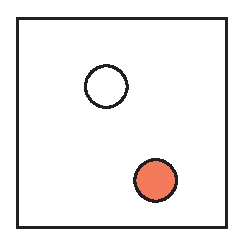
\includegraphics[width=1.5in]{sample.eps}
% \caption{Lookit! Lookit!}
%}

%% Abstract section.
\abstract{
Group-in-a-box (GIB) is a graph-drawing method designed to facilitate the visualization of the group structure of a graph.
GIB allows the user to simultaneously view group sizes and inter- and intra-group structures.
Several GIB variants have been proposed in the literature; however, their advantages and disadvantages have not been studied from the perspective of human cognition.
Therefore, herein, we used eye tracking analysis and user surveys to evaluate the user experience of four GIB variants: Squarified-Treemap GIB(ST-GIB), Croissant-and-Doughnut GIB (CD-GIB), Force-Directed GIB (FD-GIB), and Tree-Reordered GIB (TR-GIB).
We found some trade-offs among the methods for each type of user task and that FD-GIB and TR-GIB are superior than the other variants.
Although ST-GIB's results were good, links were difficult to read in this graph layout.
Eye-tracking data was gathered to determine which elements in each visualization significantly affected user experience.
The results of this study will promote the effective use of GIB to analyze networks such as social networks or web graphs.
} % end of abstract

%% ACM Computing Classification System (CCS). 
%% See <http://www.acm.org/about/class> for details.
%% We recommend the 2012 system <http://www.acm.org/about/class/class/2012>
%% For the 2012 system use the ``\CCScatTwelve'' which command takes four arguments.
%% The 1998 system <http://www.acm.org/about/class/class/2012> is still possible
%% For the 1998 system use the ``\CCScat'' which command takes four arguments.
%% In both cases the last two arguments (1998) or last three (2012) can be empty.

\CCScatlist{
  \CCScatTwelve{Human-centered computing}{Visu\-al\-iza\-tion}{Visu\-al\-iza\-tion techniques}{Graph drawings};
  \CCScatTwelve{Human-centered computing}{Visu\-al\-iza\-tion}{Visualization design and evaluation methods}{}
}

%\CCScatlist{
  %\CCScat{H.5.2}{User Interfaces}{User Interfaces}{Graphical user interfaces (GUI)}{};
  %\CCScat{H.5.m}{Information Interfaces and Presentation}{Miscellaneous}{}{}
%}

%% Copyright space is enabled by default as required by guidelines.
%% It is disabled by the 'review' option or via the following command:
% \nocopyrightspace

%%%%%%%%%%%%%%%%%%%%%%%%%%%%%%%%%%%%%%%%%%%%%%%%%%%%%%%%%%%%%%%%
%%%%%%%%%%%%%%%%%%%%%% START OF THE PAPER %%%%%%%%%%%%%%%%%%%%%%
%%%%%%%%%%%%%%%%%%%%%%%%%%%%%%%%%%%%%%%%%%%%%%%%%%%%%%%%%%%%%%%%%

\begin{document}

%% The ``\maketitle'' command must be the first command after the
%% ``\begin{document}'' command. It prepares and prints the title block.

%% the only exception to this rule is the \firstsection command
\firstsection{Introduction}

\maketitle

%% \section{Introduction} %for journal use above \firstsection{..} instead
In the field of graph drawing, numerous methods have been proposed for visualizing network data \cite{Vehlow2017VisualizingGS,doi:10.1177/1473871612455749, saket2014group}, with each method aiming at a different visualization goal.
Some methods are designed for the analysis of graphs representing real-world relationships such as social networks and web graphs.
These networks are often characterized as complex ~\cite{Newman:2010:NI:1809753} because they tend to have community structure~\cite{girvan2002community,newman2004detecting}.
A network with community structure contains groups of nodes which have dense within-group connections and sparse between-group connections.
For example, networks of Twitter accounts represent users as nodes; pairs of users that mention each other are connected with edges, which can be weighted according to the number of mentions.
In such a network, users can be divided into groups using the topology or other features of the graph.
When a network is larger or has higher density, observers may face more difficulty in understanding a graph of the network because the high numbers of nodes, edges, and groups may be cluttered.
One general method for distinguishing groups in a graph is to present nodes with different colors or shapes; however, this method is not effective for a large or dense network.
To analyze real-world data, effective visualization techniques for understanding the group structure of a network is essential.
% There are various methods to group related nodes in a network based on a feature of that such as the topology, some attributes the nodes have, or the combination of them~\cite{clauset2004finding,wakita2007finding,lloyd1982least,navlakha2009finding}.
% A topological method generates groups so that the relationships among nodes in a single group are stronger than those between nodes in different groups.
% The latter method takes some common attributes of the nodes. For example, in the case of a Twitter network, there are users' geographical locations, religions, and interests.
% General methods to illustrate groups in a graph visually discriminate them by the color or shape of nodes, which does not make groups easy to understand in a large network.

Group-in-a-box (GIB), illustrated in Figure~\ref{GIB-examples}, is a graph-drawing method designed for networks having a community structure.
Among the many available community-structured methods for visualizing graphs, GIB is well-studied and has several variants with different visualization goals~\cite{rodrigues2011group,chaturvedi2014group,onoue2017optimal}.
GIB arranges all nodes in a group into a box that has an area proportional to the number of nodes in the group such that each group can be visualized separately.
The GIB layout enables simultaneous visualization of group structures, group relationships, inter-group relationships, and the sizes of the groups in a graph.
% Specifically, it is expected that placing groups in individual boxes aids in the understanding of the information within a group.
% There are several variants of GIB layout, and each of them has a different original purpose.
Although some computational experiments~\cite{chaturvedi2014group,onoue2017optimal} have evaluated GIB variants, to the best of our knowledge, no user experiments have tested variations of the proposed approach.
Some network measures were used in the abovementioned computational experiments (e.g., the number of edge crossings) that are known to affect the readability of a graph ~\cite{468391,purchase1997aesthetic,purchase1998performance,purchase2002empirical}. Graph readability is also affected by other more-subjective factors, which are easiest to evaluate through user testing.

Therefore, we employed user testing to ascertain which GIB variant offers the most utility to users.
Study participants tested the Squarified-Treemap GIB(ST-GIB), Croissant-and-Doughnut GIB (CD-GIB), Force-Directed GIB (FD-GIB), and Tree-Reordered GIB (TR-GIB) variants.
ST-GIB uses the squarified treemap algorithm \cite{bruls2000squarified} to lay out the group boxes.
CD-GIB arranges the boxes according to the number of other boxes connected to it, which may result in less visual clutter.
A force-directed layout scheme is used to arrange the boxes in FD-GIB, whereas TR-GIB is produced by reordering boxes generated using the ST algorithm to minimize group proximity.
We implement four types of tasks in user tests designed on the basis of survey studies by Vehlow et al.~\cite{Vehlow2017VisualizingGS} and Saket et al.~\cite{saket2014group} to observe each layout's features from various perspectives.
We measured the accuracy and completion time for each task.

We also collected eye-tracking data during the tests.
Eye tracking is a technique used to record gaze data, and it is often used in the field of human--computer interaction.
Gaze data is useful for understanding task performance in our tests because the gaze data of participants can grant insight into why a specific layout achieves better results than the others~\cite{andrienko2012visual,duchowski2007eye,kurzhals2014evaluating}.
% Together with the accuracy and completion time of tasks, we also analyze eye-tracking data to reveal the differences between layouts.
Specifically, we use gaze data to understand which elements in a layout help or hinder users when performing the experimental tasks.
These elements may also have an influence on the readability of other visualization techniques.


One of our main contributions is the evaluation of four GIB layouts and the determination of the best GIB.
We assume that each GIB has advantages and disadvantages. Thus, we aim to evaluate these GIB variants through four tasks and verify which GIB is significantly superior in each task.
We also provide some evidence to support our results using the eye-tracking data to clarify which elements in a particular visualization affect the results.
Finding these elements might contribute to the improvement of both GIB and other visualization techniques.

The four GIB layout schemes have also been made available to the public. Our website provides GIB images, as well as further analysis of the networks~\cite{gibweb}.
These schemes can help researchers in analyzing their network data and may even encourage new findings.
% \vspace{-1cm}

%
\section{Related Work}
%
In this section, we review two types of related studies.
The first type concerns graph drawing methods for networks having community structure, and the second type concerns the evaluation of visualization using eye-tracking data.

\subsection{Graph-drawing Method for Group Structure}
Graph drawings are used to design a layout for complex networks.
Eades proposed a method using force-directed placement in which attractive and repulsive forces are balanced to produce an optimal equilibrium~\cite{eades84}.
This force-directed method has been widely used~\cite{Kobourov2013ForceDirectedDA}, and several approaches are also available for this purpose (see, e.g., \cite{harel2000fast,koren2003drawing,hachul2004drawing,article}).

However, the recent popularity of network visualization has led to the development of techniques specifically designed for visualizing networks with group structure.
In large-scale network data, the importance of community detection is known and several approaches have been invented, often based on a force-directed layout. One typical method to illustrate the group structure of a graph is varying the color~\cite{mcpherson2005discovering} or shape of nodes; but this method is often ineffective in real-world networks.

Vehlow et al.\ provided a survey of the visualization of group structures in graphs~\cite{Vehlow2017VisualizingGS}.
They described a taxonomy of visualization methods and tasks employed in user testing.
This visualization taxonomy is classified as follows: vertex visualization and vertex group structure.
The former represents visual grouping of nodes, either by node attributes, juxtaposition, superimposition, or embedding.
The latter depends on whether a network can be characterized by group overlapping and/or the hierarchy of the graph structure.
A node in a network with group overlapping may simultaneously belong to multiple groups.
A hierarchical network features a hierarchical structure among groups.
% The abovementioned study introduced some visualizations designed for a network with group structure for each category in the taxonomy.

The GIB layout is also a visualization for group structure; it is presented in~\cite{rodrigues2011group,chaturvedi2014group,onoue2017optimal}.
% There are 4 major variants of GIB, which we consider in this research: ST-GIB, CD-GIB, FD-GIB, and TR-GIB.
% This layout has the advantage of visualizing each group in a clearly separate way, which allows the observation of the relationship between two nodes in the same group easily.
% It can also show a group size visually with the area of a rectangular.
This method is categorized as a superimposed visualization and is best for networks without group overlapping in Vehlow's taxonomy. ST-GIB and TR-GIB can be also applied for networks with hierarchical structure.
% An example of network data in which GIB is effective is Twitter data with some groups defined with the user locations because their locations cannot overlap.
Chaturvedi et al.~\cite{chaturvedi2014group} compared three types of GIBs: ST-GIB, CD-GIB, and FD-GIB, by calculating several objective measures: edge-box overlap, percent screen space wasted, execution time, and mean group-box aspect ratio.
They also provide several case studies.
% They observed strong differences in the computational measures among the three layouts; especially, FD-GIB is good at reducing the number of edge-box overlaps but not at saving screen space.

Although such objective evaluation is effective, it is insufficient because certain hidden factors such as human cognition also influence readability. A user study in which participants use the graphs to complete multiple tasks could facilitate a more-thorough discussion of the layout's effectiveness and appropriately evaluate GIBs while considering such hidden factors.
The algorithm proposed by Didimo and Montecchiani~\cite{6295786} also produces a good layout for visualizing group structure with arranging groups in boxes; however, this looks similar to FD-GIB.
For the sake of easy comparisons, we focus on only four GIB layouts in this study.

\subsection{Evaluation through Eye Tracking}
Several studies have evaluated visualization techniques through eye tracking~\cite{burch2011evaluation,pohl2009comparing,netzel2014comparative,jianu2014display,7539393}, which have been widely used to collect gaze data and measure the participants' visual attention~\cite{andrienko2012visual,duchowski2007eye,kurzhals2014evaluating}.
Such systems are often used to analyze how well participants perform in a user study. Researchers can elicit clues about why one visualization is better than another by analyzing gaze data.

Burch et al.\ evaluated three variants of tree diagrams through eye tracking~\cite{burch2011evaluation}. 
%They gave participants a task to find the least common ancestor of a set of given nodes. They collected gaze data as well as task accuracy and completion time, and they analyzed it using techniques designed for the analysis of gaze data, such as trajectory map, heat map, and gaze flow between a pair of areas of interest (AOIs).
Their analysis of eye-tracking data explained why the task-completion results differed, as they found that the task with the layout with the least accuracy required users to look over complex cross-check trajectories.

Several studies provide guidelines on the visual analytics of eye-tracking data~\cite{andrienko2012visual,kurzhals2014evaluating,duchowski2007eye}.
Eye-tracking datasets are often very large and difficult to analyze; hence, spatiotemporal gaze data requires specific methodologies for analysis.
Burch et al.\ mentioned two methods for analyzing gaze data~\cite{Burch2013VisualTS}, focusing on either areas of interest (AOIs) or gaze trajectories.
Since early studies, researchers have known that although AOI plays a crucial role in the analysis process of eye movement data, people concentrate on interesting and informative regions of a display~\cite{yarbus1967eye}.
GIB divides the screen into boxes that are naturally regarded as AOIs. Thus, AOI analysis was also used in the present study as it is particularly in the analysis conducted herein.% For effective and meaningful analytics, it is important to know what kind of methods are most appropriate, and these studies can give researchers some hints.
% We collect gaze data during the tasks in order to reveal which elements in a visualization affect performance.
% We suppose that this study becomes more meaningful by following these analysis methods.

\section{GIB Layouts}
%{}
This section describes the four evaluated GIB variants, examples of which are shown in Figure~\ref{GIB-examples}.
Each graph in this figure has a different GIB layout, but all layouts are representations of the same network data.
As regards evaluation, Chaturvedi et al.\ have performed a computational experiment on three of these layouts: ST-GIB, CD-GIB, and FD-GIB \cite{chaturvedi2014group}.
Onoue et al.\ showed that TR-GIB is advantageous over ST-GIB in terms of computational measures \cite{onoue2017optimal}.
Our target layouts are the four abovementioned layouts which need to be evaluated from the perspective of human cognition through user experiment.
% We use the force-directed layout to draw network within a group, but it is also possible to use other methods.

\subsection{FD-GIB}
Chaturvedi et al.~\cite{chaturvedi2014group} also proposed the FD-GIB layout (Figure~\ref{GIB-examples}(c)).
In FD-GIB, the group boxes are arranged with a force-directed layout run on the whole network, with the vertices for this layout representing entire groups and the edges between them representing the links between groups.
Then, group boxes are overlaid on this initial layout.%, centered at the group's position.
FD-GIB can cause group overlaps, which are then removed using the PRISM method~\cite{gansner2008efficient}.

Chaturvedi et al.\ used the Harel--Koren fast multiscale layout~\cite{harel2002graph} to arrange the rectangles in FD-GIB, but we use the D3.js force simulation~\cite{Bostock:2011:DDD:2068462.2068631} because of its easy availability and good results.
However, as reported by Chaturvedi et al.~\cite{chaturvedi2014group}, according to experimental evaluations of several layout algorithms performed by Hachul et al.~\cite{Hachul:2005:ECF:2102325.2102348,Hachul2007LargeGraphLA}, several good options are available~\cite{harel2002graph,koren2003drawing}.
% , such as the high-dimensional embedding approach~\cite{harel2002graph} or the algebraic multi-grid method~\cite{koren2003drawing}.

This layout clearly displays the aggregate topology, but it uses more screen space.
The area of each group must be smaller than that of the other layouts; hence, the relationships within a single group are more difficult to observe. However, this layout can maintain a consistent aspect ratio because of which participants can easily recognize the size differences between boxes.

\subsection{TR-GIB}
Onoue et al.\ developed TR-GIB to minimize the weighted sum of distances between groups by reordering the sibling nodes laid out by ST-GIB~\cite{onoue2017optimal}.
An example of this layout is shown in Figure~\ref{GIB-examples}(d).
This method is visually similar to ST-GIB, but the tiles are reordered by solving an optimization problem to reduce the total length of the links between groups.
As treemaps, such as ST-GIB, have a tree-like structure, vertices with the same depth in a tree can be reordered.
The shorter edges in TR-GIB reduce the number of edge crossings, thereby improving the readability of the graph.
% Specifically, the sum of the distances between two groups is weighted according to the number of edges between the two groups, and this sum is taken as the group proximity.
We expect this layout to have the advantages of ST-GIB (i.e., good aspect ratio and screen efficiency) with an additional advantage of fewer edge overlaps.

\section{Additional Experiment}
In this experiment, we focus on FD-GIB and TR-GIB which achieve good result.
As we found that they had trade-off because of their visual or algorithmic features, we suppose that TR-GIB might get better result with more complex task in experiment.
We also had a limitation in the last study that the data size is fixed and not so big.
In the recent graph drawing, the data scalability is popular topic which we have to work on.
When data size is big, the readability of a graph drawing method observed in with smaller data might be disappeared since many nodes and edges cause visual clutter as well as unexpected foctors that do not exist in the case with smaller data set.
Therefore, we aim to figure out the effectiveness of FD-GIB and TR-GIB more in detail, and also try to reveal their data scalabilities.

our contribution is to figure out the data scalability of FD-GIB and TR-GIB using a complex task that is similar operation as actual data exploring.
Knowledge about the effectiveness of them especially for big data let us utilize them appropriately and analyze recent meaningful big data.
Eye tracking is used to record the gaze data of participants during experiment.
We expect that we could get several discoveries by analyzing that data; specifically, what elements in FD-GIB and TR-GIB affect the readability of a graph.

\section{レイアウト}
レイアウトは

\section{Data Generation}
Since we focus the data scalability of GIBs in this study, 


%\bibliographystyle{abbrv}
\bibliographystyle{abbrv-doi}
%\bibliographystyle{abbrv-doi-narrow}
%\bibliographystyle{abbrv-doi-hyperref}
%\bibliographystyle{abbrv-doi-hyperref-narrow}

\bibliography{template}
\end{document}A
